\documentclass[11pt]{article}
\usepackage{euscript}

\usepackage{amsmath}
\usepackage{amsthm}
\usepackage{amssymb}
\usepackage{mathtools}
\DeclarePairedDelimiter{\ceil}{\lceil}{\rceil}
\usepackage{epsfig}
\usepackage{xspace}
\usepackage{color}
\usepackage{url}
\usepackage{enumerate}
\usepackage{listings}

%%%%%%%  For drawing trees  %%%%%%%%%
\usepackage{tikz}
\usetikzlibrary{calc, shapes, backgrounds}

%%%%%%%%%%%%%%%%%%%%%%%%%%%%%%%%%
\setlength{\textheight}{9in}
\setlength{\topmargin}{-0.600in}
\setlength{\headheight}{0.2in}
\setlength{\headsep}{0.250in}
\setlength{\footskip}{0.5in}
\flushbottom
\setlength{\textwidth}{6.5in}
\setlength{\oddsidemargin}{0in}
\setlength{\evensidemargin}{0in}
\setlength{\columnsep}{2pc}
\setlength{\parindent}{1em}
%%%%%%%%%%%%%%%%%%%%%%%%%%%%%%%%%

\newcommand{\eps}{\varepsilon}

\renewcommand{\c}[1]{\ensuremath{\EuScript{#1}}}
\renewcommand{\b}[1]{\ensuremath{\mathbb{#1}}}
\newcommand{\s}[1]{\textsf{#1}}

\newcommand{\E}{\textbf{\textsf{E}}}
\renewcommand{\Pr}{\textbf{\textsf{Pr}}}


\title{Asmt 1: Hash Functions and PAC Algorithms}
\author{Yulong Liang (u1143816)}

\begin{document}
\maketitle


\section{Birthday Paradox (30 points)}

\begin{enumerate}[A]
\item In the first simulation, it took 68 trials to reach a collision, i.e., $k = 68$.
\item The cumulative density plot is shown below:
\begin{figure}[h]
\centering{
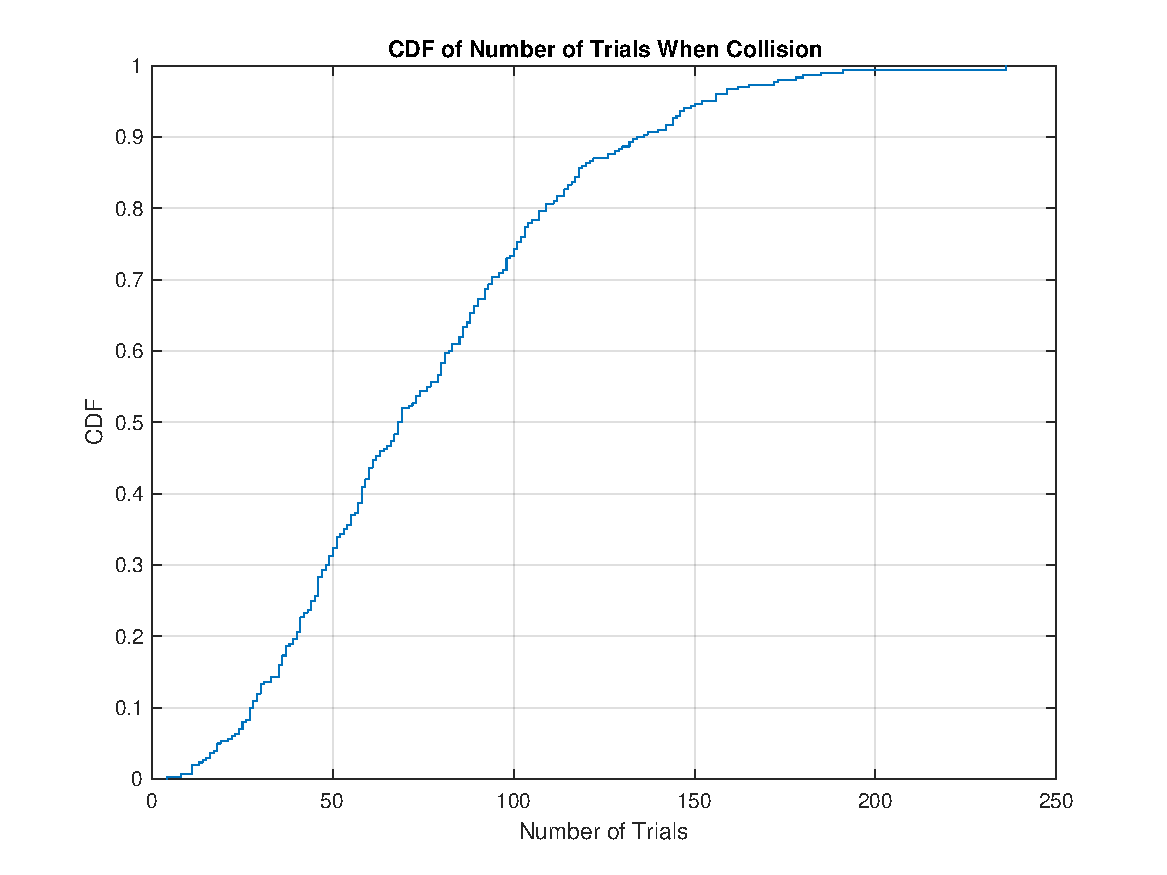
\includegraphics[width=.6\linewidth]{cdf.pdf}
}
\caption{Cumulative Density Plot of Number of Trials When Collision}
\label{fig:name}
\end{figure}

\item The empirical expected number is $\mathbb{E} = 75.9600$.
\item First I implemented the experiment with \textbf{Matlab}, using \texttt{containers.Map} and a \texttt{vector} of size n, i.e., a normal array  respectively. Then I switched to \textbf{Python} using a \texttt{python list}, a \texttt{numpy array} and a \texttt{python set} respectively to compare the speed between the two languages.
For the experiment of $n=4000$ and $m=300$, the runtime is as follows,
\begin{table}[h]
\centering
\begin{tabular}{ccc}
Language & Data Type & Run Time\\
\hline
Matlab & Map & 0.4528\\
Matlab & Vector & 0.0430\\
Python & Numpy Array & 0.0591\\
Python & List & 0.0491\\
Python & Set & 0.0432\\
\end{tabular}
\end{table}\\
Below is a plot of the run time of the implementation with \texttt{Matlab Vector} for $m=300$, $m=2000$, $m=10000$\\
\begin{figure}[h]
\centering{
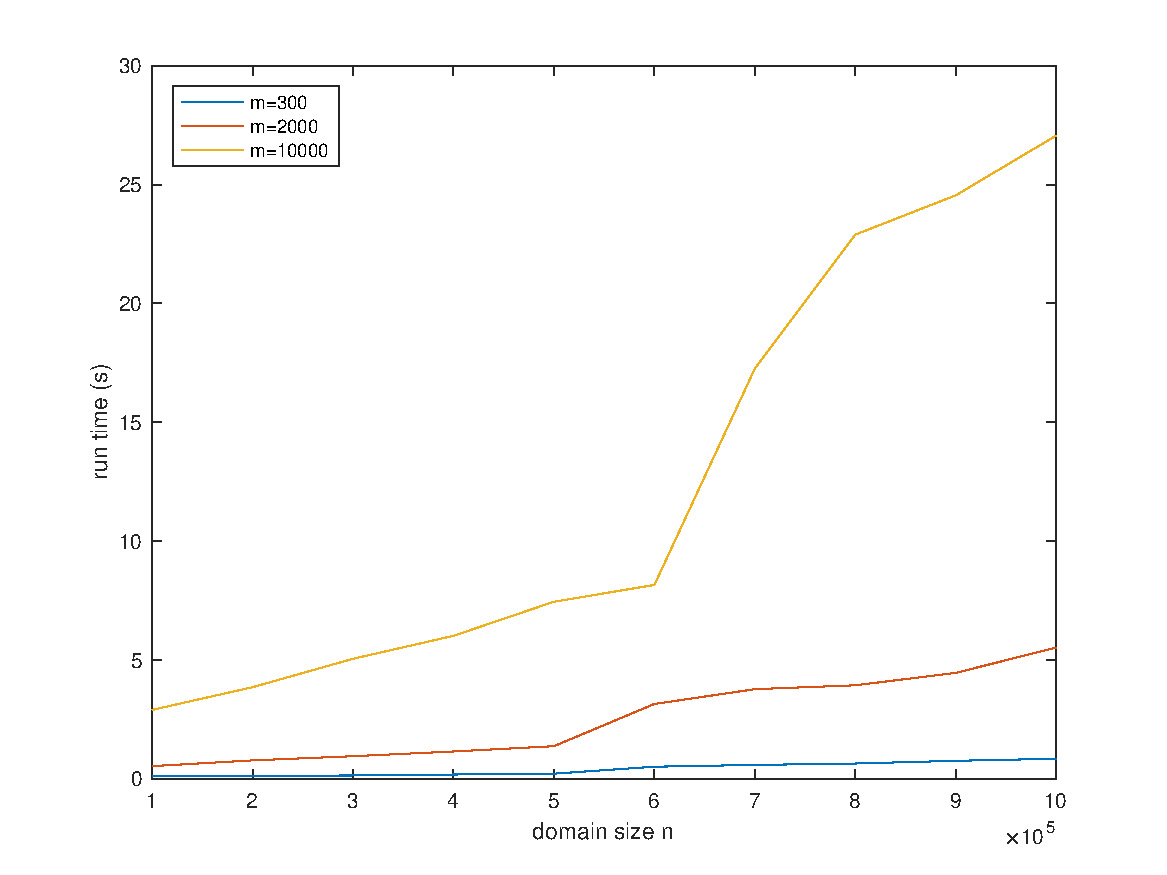
\includegraphics[width=.6\linewidth]{bp.pdf}
}
\caption{Run Time of the Implementation with \texttt{Matlab Vector}}
\label{fig:name}
\end{figure}\\
The codes are as follows,
\begin{lstlisting}[language=Matlab]
function k = birthdaySimulatora2(n)
    map = zeros(1,n);
    k = 0;
    while 1
        x = randi(n);
        if map(x) == 1
            return;
        else
            map(x) = 1;
            k = k + 1;
        end
    end
end
\end{lstlisting}
\end{enumerate}

\newpage
\section{ Coupon Collectors (30 points)}

\begin{enumerate}[A]
\item In the first simulation, it took 1367 trials to cover all the numbers, i.e., $k = 1367$.
\item The cumulative density plot is shown below:
\begin{figure}[h]
\centering{
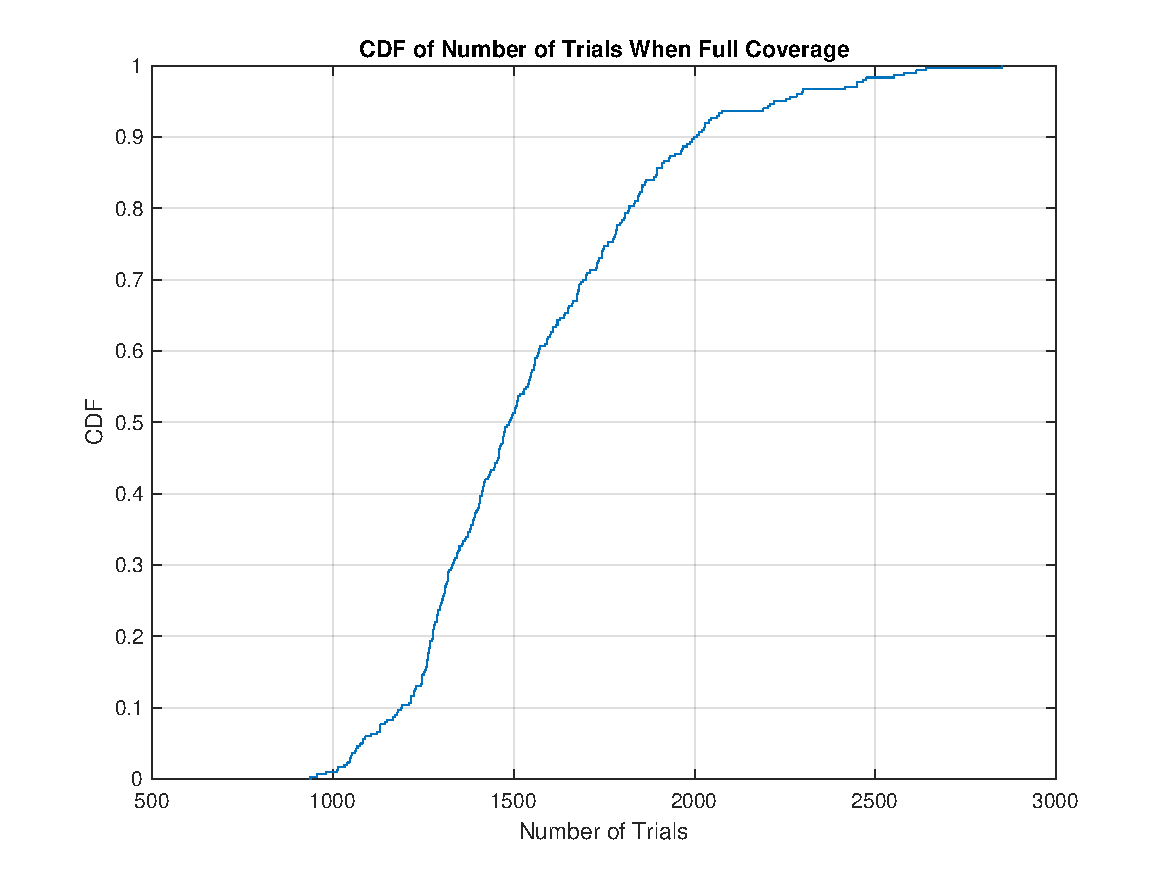
\includegraphics[width=.6\linewidth]{cdf2.pdf}
}
\caption{Cumulative Density Plot of Number of Trials When Full Coverage}
\label{fig:name}
\end{figure}

\item The empirical expected number is $\mathbb{E} = 1555.7233$.
\item First I implemented the experiment with \textbf{Matlab}, using \texttt{containers.Map} and a \texttt{vector} of size n respectively. Then I switched to \textbf{Python} using a \texttt{python list}, a \texttt{numpy array} and a \texttt{python set} respectively to compare the speed between the two languages.
For the experiment of $n=250$ and $m=300$, the run time is as follows,
\begin{table}[h]
\centering
\begin{tabular}{ccc}
Language & Data Type & Run Time\\
\hline
Matlab & Map & 3.3359\\
Matlab & Vector & 0.9666\\
Python & Numpy Array & 0.6793\\
Python & List &  0.5535\\
Python & Set & 0.5349
\end{tabular}
\end{table}\\
Below is a plot of the run time of the implementation with \texttt{Matlab Vector} for $m=300$, $m=1000$, $m=5000$,
\begin{figure}[h]
\centering{
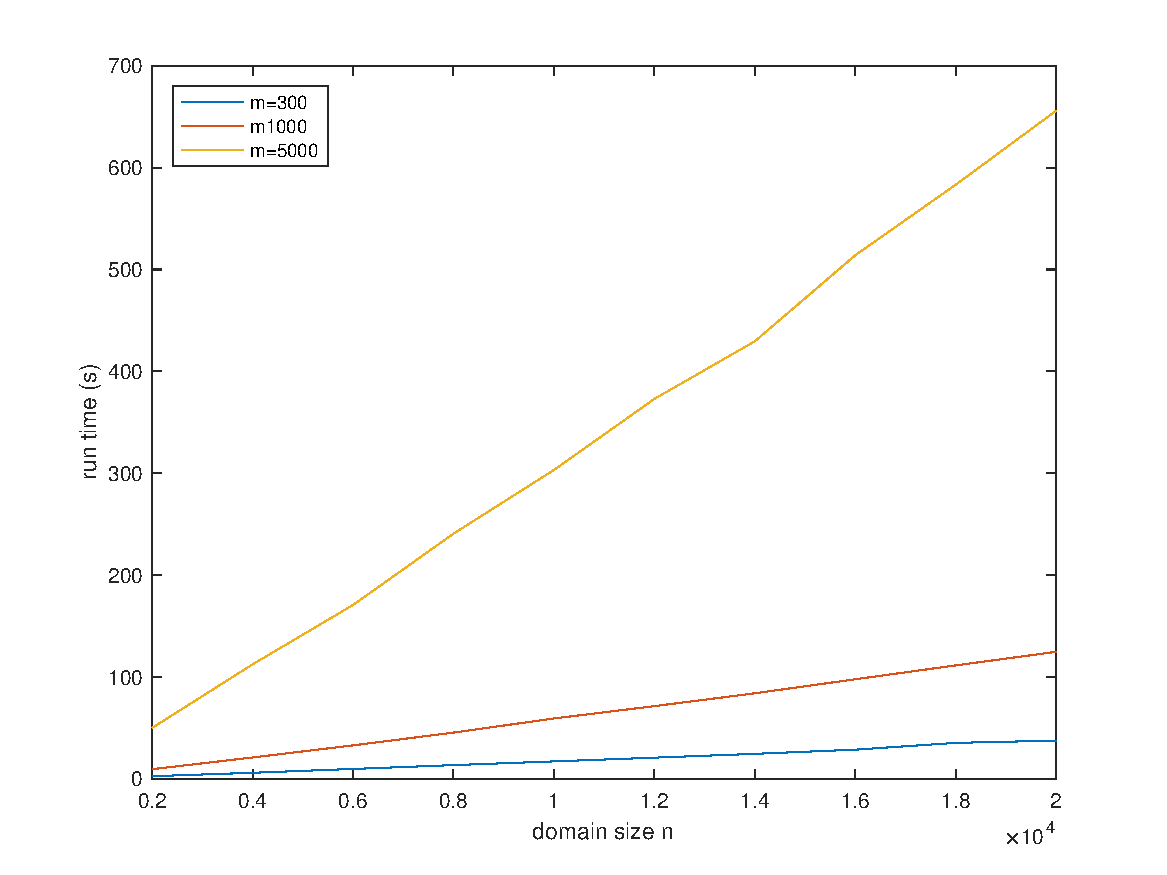
\includegraphics[width=.6\linewidth]{cc.pdf}
}
\caption{Run Time of the Implementation with \texttt{Matlab Vector}}
\label{fig:name}
\end{figure}

\newpage
The codes are as follows,
\begin{lstlisting}[language=Matlab]
function k = couponSimulatora2(n)
    map = ones(1,n);
    k = 0;
    length = n;
    while length > 0
        k = k + 1;
        x = randi(n);
        if map(x) == 0
            continue;
        else
            map(x) = 0;
            length = length - 1;
        end
    end
end
\end{lstlisting}
\end{enumerate}

\section{Comparing Experiments to Analysis (24 points)}

\begin{enumerate}[A]
\item The analytical expected number is $\mathbb{E}=75$, which is very near to the empirical expected number $\mathbb{E} = 75.9600$.\\
The formula I used is:
\[
\frac{n}{n} \cdot \frac{n-1}{n} \cdot \frac{n-2}{n} \cdot \cdots \cdot \frac{n-(k-1)}{n} = \prod_{i=1}^{k-1}\frac{n-i}{n} \leq 0.5
\]
The solution to the formula is:
\[
k \geq 75
\]
The strategy of coding is using a for loop to calculate the product from k = 1 when the product is 1 until the product is less than or equal to 0.5. Then return the value of k.

\item The analytical expected number is $\mathbb{E}=1525.1688$, which is very near to the empirical expected number $\mathbb{E} = 1555.7233$.\\
The formula I used is:
\[
T=\sum_{i=1}^nt_i=\sum_{i=1}^n\frac{n}{n-i+1}=n\sum_{i=1}^n\frac{1}{i}=250\cdot\sum_{i=1}^{250}\frac{1}{i}\approx1525.1688
\]
The strategy of coding is using a for loop to calculate the summation.
\end{enumerate}

\section{Random Numbers (16 points)}
\begin{enumerate}[A]
\item Call \texttt{rand-bit()} function for 10 times, which will provide 10 random binary numbers. The conbination of the 10 binary numbers will form a random integer a between 0 and 1023. Let $a+1$ be the final result.
\item Using the method of 4A, the algorithm will generate random numbers in $[1024]$. If the number is in $[1000]$, the algorithm will finish and return the number it generated. If the number is in $[1001, 1024]$, the algorithm will generate another random number in $[1024]$. The algorithm will run iteratively until it generates a number in $[1000]$.\\
For each generation, the probability of success is $\cfrac{1000}{1024}=0.9765625$, the probability of failure is $\cfrac{24}{1024}=0.0234375$. The expected number of generations is,
\[\mathbb{E} = 1\cdot p+2\cdot pq+3\cdot pq^2 \cdot i\cdot qp^{i-1}\cdots=\cfrac{1}{p}=1.024
\]
\item The expected number of calls of \texttt{rand-bit()} made for a random number in domain $[n]$ is, 
\[\frac{2^{\ceil{\log_2n}}}{n}\cdot \ceil{\log_2n}\]
\end{enumerate}

\section{BONUS : PAC Bounds (2 points)}
From the context, $\mu$ and $\cfrac{1}{n}$ are the maximum and expectation value of the frequency of value i respectively.
\begin{gather}
\mu=max(\frac{f_i}{k})\\
\frac{1}{n}=\mathbb{E}(\frac{f_i}{k})
\end{gather}
Assume we have a set of $k$ iid random variables $\{X_1, X_2, \cdots, X_k\}$, $X_i \in \{0,1\}$ for each $i \in [k]$. Then,
\begin{gather}
A=\frac{1}{k}\sum_{i=1}^{k}X_i=\frac{f_i}{k}\\
-1\leq X_i\leq1\quad\Rightarrow\quad\Delta=1
\end{gather}
Substituting (1)(2)(3)(4) into the Chernoff-Hoeffding inequality,
\begin{gather}
\Pr[|A-E[A]|>\epsilon]\le2\cdot \exp(\frac{-r\epsilon^2}{2\Delta^2})\\
\Pr[|\mu-\frac{1}{n}|>\epsilon]\le2\cdot \exp(\frac{-k\epsilon^2}{2})
\end{gather}
In order that the right part of the inequality equals 0.02,
\begin{gather}
2\cdot \exp(\frac{-k\epsilon^2}{2})=0.02\\
k=\frac{2\ln100}{\epsilon^2}
\end{gather}
In order that the right part of the inequality equals 0.002,
\begin{gather}
2\cdot \exp(\frac{-k\epsilon^2}{2})=0.002\\
k=\frac{2\ln1000}{\epsilon^2}
\end{gather}
Thus, k need to be great than or equal to $\cfrac{2\ln100}{\epsilon^2}$ for the probability of failure to be less than or equal to 0.02 and $\cfrac{2\ln1000}{\epsilon^2}$ for the probability of failure to be less than or equal to 0.002.

\end{document}
